\chapter{Requerimientos}
\label{chap:requerimientos}

\observacion{Unificar juego y videojuego}

Realizada la propuesta de aplicación en la que se centra este trabajo de grado,
se describe los requerimientos necesarios para que la misma cumpla su objetivo
pedagógico.

Esta capítulo además se centra en los objetivos pedagógicos que se desean
obtener, el cual es un paso necesario para poder realizar el flujo de desarrollo
descrito en~\ref{sec:desarrollo}.

Primeramente se definen los criterios para definir cuales procedimientos pueden
ser simulados, luego se describen los procedimientos seleccionados, con los
detalles de los mismos y las competencias básicas que están definidas en su plan
de estudio. Se describe el aspecto de la bioseguridad, que es un aspecto
fundamental de todo procedimiento de enfermería.

A fin de determinar el alcance de la solución, se describen hipótesis acerca de
lo que es necesario incluir, cuales detalles deben ser cubiertos por completo,
cuales son necesarios sin mucho detalle y cuales pueden ser dejados de lado. 

El último aspecto tratado en este capítulo es el de los requisitos transversales
que debe cumplir la solución, como aspectos de jugabilidad, como manipulación de
la cámara, interfaz, etc, así como aspectos pedagógicos, como la
retroalimentación, muestra de información y progreso.

%! TEX root = ../main.tex
\section{Definición de criterios}
\label{sec:criterios}

Se realizaron varias reuniones con la coordinadora de la carrera de Licenciatura
en Enfermería del \Gls{iab} y profesores encargados de las prácticas de
laboratorio y campo de diversas materias de la carrera. De estas reuniones, y
del plan de estudios de la carrera de enfermería, se extraen procedimientos que
pueden ser simulados, cuya aceptación y validación son realizados por  
profesores del área de enfermería del \Gls{iab}.

De los procedimientos evaluados y discutidos se eligen dos ya que la variedad y
cantidad de procedimientos de enfermería existentes es muy alta e incluirlos
todos a la solución está fuera del alcance de este trabajo. Los principales
criterios para la selección de los procedimientos son los siguientes:

\begin{itemize}

    \item \textbf{Deben adecuarse a las limitaciones de la tecnología} 

    Escenarios que requieren la simulación de órganos internos, psicología
    humana, etc, pueden requerir una complejidad adicional a la hora de
    implementar la simulación, complejidad que escapa al alcance del presente
    trabajo.

    \item \textbf{Deben de ser de utilidad para los alumnos} 
    
    Deben ser procedimientos comunes en la vida profesional de un enfermero, o
    que no sea posible realizar practicas frecuentes. 

    Al ser una profesión relacionada con la salud, existen múltiples factores
    que dificultan las prácticas de enfermería, como la salud del paciente, la
    salud del profesional, enfermedades o procedimientos poco frecuentes, etc.

\item \textbf{Los procedimientos seleccionados no deben ser complejos ni
        extensos}. 

    Las simulaciones cortas permiten poder ser utilizadas en cualquier momento,
    sin ser interrumpidas. En cuanto al nivel de detalle del entorno, los
    entornos complejos dificultan la atención del
    usuario\cite{videojuegos:gonzaleztardon}, por ello, los factores que son
    simulados deben ser los suficientes para permitir al usuario sentirse dentro
    de la misma, pero no deberían ser muy complejos, sino, el usuario desviaría su
    atención hacia los detalles.

\item \textbf{Deben tener pasos definidos}
    
    Si el procedimiento tiene un objetivo claro, y un conjunto de pasos
    previamente definidos y previsibles, se facilita la aceptación del mismo por
    los profesores, es decir, es más fácil realizar una validación de la
    simulación.

    Hay un compromiso entre la validación de la simulación y la libertad de
    exploración de los usuarios, el escenario elegido debe tener pasos
    definidos, pero a la vez debe permitir al alumno explorar el escenario y
    tomar caminos alternativos.

\item \textbf{Deben ser difíciles de representar con realismo en un aula o
        laboratorio}

    Los laboratorios del \Gls{iab} cuentan con diferentes herramientas que
    facilitan ciertos procedimientos, pero estos no pueden abarcar el amplio
    rango que cubren los procedimientos de enfermería, por ello se debería
    elegir un procedimiento que muestre las ventajas de la tecnología y técnicas
    propuestas, el procedimiento tiene que representar un desafío a las técnicas
    actuales, este desafío puede ser 
    \begin{enumerate*}[label=\itshape\alph*\upshape.]
    \item técnico, como falta de herramientas, como equipos médicos, maniquíes,
        etc, o,
    \item humano, como falta de pacientes con la patología deseada.
    \end{enumerate*}
    
\end{itemize}

%! TEX root = ../main.tex
\section{Selección de procedimientos}
\label{sec:seleccion_escenas}

Con los criterios definidos \fixme{se seleccionaron}{tiempo} dos procedimientos de enfermería,
los cuales serán incluidos en la solución. A continuación se fundamentan
\fixme{tales}{?} elecciones y se entra en detalle acerca de los procedimientos
seleccionados.

%Estos procedimientos son incluidos en la solución creando escenarios dentro del
%videojuego que permitan realizarlos, es así que cada procedimiento es
%representado con escenarios y escenas diferentes.

\subsection{Extracción de muestras de sangre}
\label{sec:hemocultivo}

El procedimiento denominado \emph{Punción venosa} es utilizado frecuentemente
para extraer muestras de sangre, es un procedimiento invasivo que ofrece un
medio directo de acceso al sistema vascular. 

La frecuencia con la que se lo utiliza esta relacionado a su utilidad para
análisis de rutina, los enfermeros lo realizan a diario y es similar a otros
procedimientos como la puesta de una vía intravenosa.

El procedimiento se puede resumir en el proceso de punzar con una jeringa el
brazo al paciente, extraer sangre y retirarla. Si bien estos pasos pueden
parecer sencillos, existen una gran cantidad de factores que definen si el
procedimiento fue realizado correctamente, entre ellas podemos encontrar a
factores de bioseguridad\footnote{La bioseguridad es la aplicación de
    conocimientos, técnicas y equipamientos para prevenir a personas,
    laboratorios, áreas hospitalarias y medio ambiente de la exposición a
    agentes potencialmente infecciosos o considerados de riesgo biológico.},
como la esterilización correcta de los materiales; sociales, como la explicación
correcta del procedimiento al paciente, etc.

Este procedimiento es considerado como uno de los apropiados de acuerdo a la
apreciación de los profesionales del \Gls{iab}, además: 

\begin{itemize}
\item El mismo posee pasos bien definidos que deben ser seguidos por el
    profesional de enfermería.
\item La complejidad del procedimiento no es muy alta, sus pasos son
    susceptibles de equivocaciones, especialmente en lo que se refiere a la
    bioseguridad. 
\end{itemize}



\subsubsection{Evaluación al alumno}

% Ver si esta bien explicar esta sección, o ir nomas al grano
\fixme{En este punto se explican las}{mejorar} competencias básicas de este
procedimiento con respecto al plan de estudio de los estudiantes de enfermería
del \Gls{iab} y los criterios relacionados al procedimiento según la planilla de
práctica que poseen los profesores instructores para evaluar al alumno.

La competencia básica que engloba al procedimiento de extracción de sangres es:

\begin{itemize}
\item Ayudar en procedimientos invasivos
\end{itemize}

Los elementos que son almacenados en la planilla de los instructores, son:
%\pregunta{Esto fue extraído de planilla del instructor, se puede poner una
%referencia la anexo}
% RESPUESTA SÍ

\begin{itemize}
\item Informe al paciente acerca del procedimiento que va a ser
    realizado.
\item Preparación de material para la técnica aséptica.
\item Lavado de manos.
\item Calzado de guantes, chaleco estéril, tapaboca y gorro.
\item Preparación de campo.
\item Punción del brazo, extracción de sangre, compresión de zona de punción.
\item Cambio de aguja.
\item Introducción de la muestra en un frasco preparado para tal efecto.
\item Retiro de materiales y equipo de protección personal.
\item Etiquetado y envío a laboratorio.
\end{itemize}

Es decir, estos son los criterios que debe cumplir cualquier estudiante
para poder aprobar la práctica.

\subsubsection{Protocolo del procedimiento}
\label{sec:hemocultivo_protocolo}

\observacion{Muy seco}


\observacion{Sujeto, verbo y predicado, La siguiente sección comprende todos los
    pasos}

La descripción formal del procedimiento, con todos los pasos necesarios
para poder llevar a cabo los criterios requeridos según~\cite{oms:extraccion}
y los profesores del \Gls{iab}, se observan en la~\ref{fig:proc_hemocultivo}, y
son los siguientes:

\begin{figure}
\centering
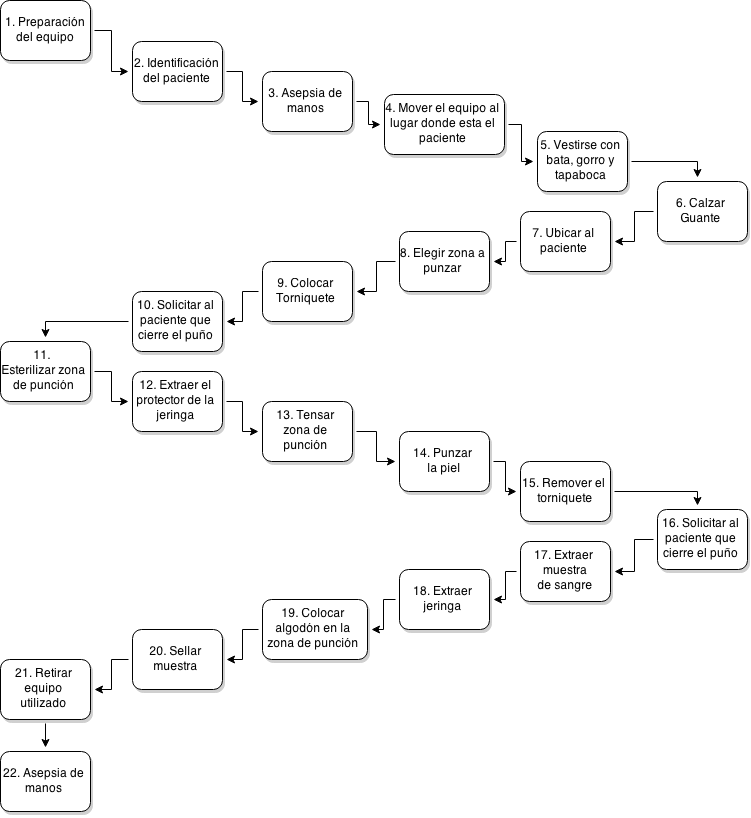
\includegraphics[scale=0.5]{requerimientos/images/hemocultivo.png}
\caption{Procedimiento de extracción de sangre.}
\label{fig:proc_hemocultivo}
\observacion{Se explica en algún lugar que no es necesariamente lineal? Por que
    se simplifica acá?}
\end{figure}

\begin{enumerate}
\item Preparar el equipo, lo que incluye seleccionar la jeringa adecuada.
\item Identificar al paciente, presentarse y explicarle el procedimiento que va
    a ser realizado.
\item Asepsia de las manos.
\item Llevar el equipo a la unidad en donde se encuentra el paciente.
\item Vestirse con bata estéril, tapaboca y gorro.
\item Calzarse los guantes.
\item Ubicar al paciente en posición adecuada, esto es, el brazo debe estar
    extendido y lo mas relajado posible.
\item Elegir la zona a puncionar, para ello se debe palpar la vena para
    averiguar sus características.
\item Colocar el torniquete, 6 a 10 centímetros por encima de la zona de
    punción.
\item Solicitar al paciente que cierre el puño.
\item Esterilizar la zona de punción.
\item Extraer el protector de la aguja.
\item Tensar la zona de punción.
\item Puncionar la piel con la aguja hacia arriba. La aguja se introduce con un
    ángulo de $10$ a $20$ grados.
\item Remover el torniquete.
\item Solicitar la apertura del puño.
\item Extraer la muestra de sangre necesaria.
\item Presionar y extraer la aguja.
\item Colocar algodón con alcohol en el punto de punción.
\item Sellar la muestra y enviarlo a su destinatario.
\item Retirar el equipo utilizado, incluyendo bata, tapaboca, gorro y guantes.
\item Asepsia de las manos.
\end{enumerate}

\subsection{Valoración de la escala de Glasgow}
\label{sec:glasgow}

La escala de Glasgow es utilizada como una herramienta de valoración objetiva
del estado de conciencia de pacientes en estado crítico\cite{protocolo}. La
escala consiste en la evaluación de tres criterios de observación clínica,
los cuales son: 
\begin{enumerate*}[label=\itshape\alph*\upshape.]
\item la respuesta ocular
\item la respuesta verbal, y
\item la respuesta motora.
\end{enumerate*}

\begin{table}[!hbt]
\centering
\begin{tabular}{llr}
\toprule
\textbf{Severidad} & 
\textbf{Puntuación} \\ 
\midrule
 Leve & 13 a 15 \\
 Moderado & 9 a 12 \\
 Grave & 3 a 8 \\
\bottomrule
\end{tabular}
\caption{Escala de valoración del estado del paciente\cite{helmick2007mild}.}
\label{tab:seleccion_glasgow_estado}
\end{table}

El puntaje que determina el estado del paciente se obtiene sumando la valoración
de cada una de las respuestas, en la figura~\ref{tab:seleccion_glasgow_estado}
se observan los posibles diagnósticos. A la vez cada respuesta se evalúa
mediante una escala independiente una de otra, donde cada respuesta se puntúa
con un número\cite{glasgow:doc}, los valores de cada respuesta se observan en las
tablas~\ref{tab:seleccion_glasgow_respuestas_ocular},~\ref{tab:seleccion_glasgow_respuestas_motor}
y~\ref{tab:seleccion_glasgow_respuestas_verbal}.

\begin{table}[!hbt]
\centering
\begin{tabular}{lr}
\toprule
\textbf{Apertura ocular} & \textbf{Valor} \\
\midrule
Espontánea & 4 \\
Al hablar & 3 \\
Al dolor & 2 \\
Ausente & 1 \\
\bottomrule
\end{tabular}
\caption{Valoración de las distintas respuestas en la escala de Glasgow,
    respecto a la reacción ocular}
\label{tab:seleccion_glasgow_respuestas_ocular}
\end{table}

\begin{table}[!hbt]
\centering
\begin{tabular}{lr}
\toprule
\textbf{Respuesta motora} & \textbf{Valor} \\
\midrule
Obedece & 6 \\
Localiza & 5 \\
Retira & 4 \\
Flexión anormal & 3 \\
Extiende & 2 \\
Ausente & 1 \\
\bottomrule
\end{tabular}
\caption{Valoración de las distintas respuestas en la escala de Glasgow,
    referentes a las respuestas motoras}
\label{tab:seleccion_glasgow_respuestas_motor}
\end{table}

\begin{table}[!hbt]
\centering
\begin{tabular}{lr}
\toprule
\textbf{Respuesta verbal} & \textbf{Valor} \\
\midrule
Orientada & 5 \\
Confusa & 4 \\
Palabras inapropiadas & 3 \\
Palabras incomprensibles & 2 \\
Ausente & 1 \\
\bottomrule
\end{tabular}
\caption{Valoración de las distintas respuestas en la escala de Glasgow
    referentes a la respuesta verbal}
\label{tab:seleccion_glasgow_respuestas_verbal}
\end{table}

El procedimiento se utiliza cuando existe un paciente con un estado de
conciencia indefinido, normalmente después de un accidente donde el paciente
recibió un traumatismo severo. El profesional que se encarga de evaluar debe
verificar el estado del paciente mediante
\begin{enumerate*}[label=\itshape\alph*\upshape.]
\item preguntas sencillas,
\item estímulos, e
\item inspecciones de partes del cuerpo.
\end{enumerate*}. 
Una vez que se obtiene una valoración individual para los aspectos
motor, ocular y visual del paciente, se obtiene la suma de las valoraciones y se
obtiene un puntaje para el estado del paciente.

El procedimiento de diagnóstico utilizando la escala de Glasgow es considerado
como uno de los apropiados para la solución propuesta ya que:

% Recheckear esto
\begin{itemize}
\item Permite la exploración del entorno pues hay diferentes formas de evaluar cada
    estado del paciente.
\item Es rara vez utilizado, pues las condiciones necesarias para que un paciente 
    requiera que se le realice este procedimiento son críticas, son
    escasas las oportunidades presentadas a los estudiantes durante sus
    prácticas de campo. 
\item La cantidad de reacciones que evalúa el procedimiento es muy alta,
    así, es difícil que un alumno pueda evaluar todos los posibles estados en
    sus prácticas de campo.
\item No es un procedimiento complejo, pues no requiere la manipulación de
    elementos, aún así requiere pericia y debe ser realizado en el menor tiempo
    posible.
\end{itemize}


\subsubsection{Evaluación al alumno}

\fixme{Se describen}{Mejorar} las competencias básicas de \enquote{Evaluación
    del alumno utilizando la escala de Glasgow} según el plan de estudios de los
estudiantes de enfermería del \Gls{iab}, la planilla de práctica que poseen los
instructores, el protocolo para llevar a cabo el procedimiento
según~\cite{protocolo} y los profesores del \Gls{iab}.

La competencia básica que incluye a la evaluación del paciente mediante la
escala de Glasgow es:

\begin{itemize}
\item Identificar actividades de cuidados según problemas urgentes principales.
\end{itemize}

En el gráfico~\ref{fig:proc_glasgow} se observan los pasos necesarios para
realizar la evaluación utilizando la escala de Glasgow\cite{protocolo}. Dentro del
procedimiento definido en la práctica profesional los criterios son:

\begin{figure}
\centering
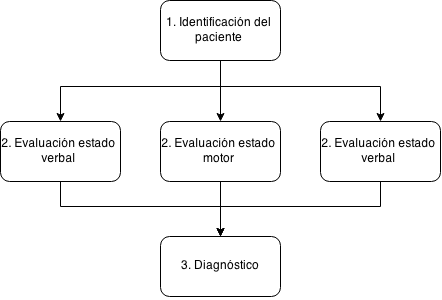
\includegraphics[scale=0.5]{requerimientos/images/glasgow.png}
\caption{Evaluación de Glasgow.}
\label{fig:proc_glasgow}
\end{figure}

\begin{itemize}
\item Control de signos vitales.
\item Inspección cefalocaudal, 
\item Evaluación utilizando escala de Glasgow.
\item Preparación del equipo según prioridad del problema
\item Analizar su participación en las actividades.
\item Fundamenta científicamente sus decisiones.
\end{itemize}

Se observa que el punto \enquote{Evaluación utilizando escala de Glasgow}, es un
paso necesario para la evaluación inicial de un paciente en estado crítico.

\subsubsection{Protocolo del procedimiento}
\label{sec:glasgow_protocolo}
\observacion{Ver tesis de parra para ver como se referencia?}

El protocolo del procedimiento, según~\cite{protocolo} y los profesores del \Gls{iab}
es:

\begin{enumerate}
\item Preparación del material
\item Preparación del paciente: comprobar su identidad, mantener una ambiente
    tranquilo evitando interrupciones, requerir la atención del paciente.
\item Colocar al paciente en posición cómoda.
\item Medir la apertura ocular.
\item Evaluar la respuesta motora.
\item Medir la respuesta verbal.
\item Registrar la puntuación final obtenida.
\end{enumerate}

\section{Alcance de la simulación}
\label{sec:alcance}

Para representar los procedimientos seleccionados y descritos en la
sección\ref{sec:seleccion_escenas}, estos deben ser presentados dentro de
escenarios distintos con los elementos necesarios para poder llevarlos a cabo.
Sin embargo, por limitaciones técnicas, tecnológicas y de tiempo, no es posible
realizar una simulación de todos los pasos requeridos.

\observacion{Más énfasis en el hecho que distrae a la parte pedagógica}
Según~\cite{videojuegos:gonzaleztardon}, existe un compromiso visible entre
realismo y credibilidad, tomando en cuenta que uno de los objetivos de la
solución es la presentación de situaciones simplificadas que permitan transmitir
conocimiento, mientras más realismo exista, más detalles existirán y por
consiguiente, los usuarios tendrán que concentrarse en un mayor número de
detalles, lo que resulta contraproducente con el objetivo de la
solución\cite{videojuegos:gonzaleztardon}. Los criterios e hipótesis que se 
describirán a continuación sirven para acotar el
alcance de la simulación, definen qué se simulará y cual es del detalle
necesario para alcanzar las competencias básicas.

\fixme{A continuación se fundamentan por qué ciertos pasos serán simulados,
    representados o no simulados dentro de la solución basados en limitaciones e
    hipótesis asumidas.}{Mover esto abajo de factores limitantes}

Cada uno de los pasos están agrupados de acuerdo a cada uno de estos aspectos.

\subsection{Factores limitantes}

Se refieren a cada uno de los aspectos que determinan si un paso 
será simulado dentro de la solución. Se clasifican en tres: limitaciones técnicas, 
importancia y facilidad de realización. Estos tres aspectos que influyen en qué partes 
se simularán y qué partes se omitirán, se detallan a continuación.

\observacion{No empezar con un ejemplo.}
\begin{itemize}
\item  \textbf{Limitaciones técnicas}: 
    
    Acciones como la simulación del agua (necesarios para el lavado de manos),
    requieren de requisitos de hardware avanzados y un tiempo considerable de
    desarrollo. Las acciones que escapan al alcance del hardware, del software o
    de tiempo de los desarrolladores no son simuladas. 
    \observacio{Reformular capítulo anterior}
        
    Los pasos del procedimiento de extracción de sangre que no se simularán por 
    limitaciones técnicas son:
    \begin{itemize}
        \item Tensar la zona de punción.
        \item Ángulo de punción.
        \item Presionar el brazo en el momento en el que se introduce la jeringa.
    \end{itemize}
    
    
\item  \fixme{Importancia}{de qué?} 

    No todos los pasos definidos en el procedimiento        
    oficial son \fixme{necesarios}{mandatorios} de simular, por ejemplo, la
    colocación de los elementos cerca del lugar de trabajo, es un paso necesario
    en el procedimiento, pero es considerado un paso poco importante y fácil de
    realizar.

    La importancia es evaluada por profesionales del \Gls{iab}, los
    cuales dieron su apreciación acerca de cada aspecto simulado, el mismo
    es tenido en cuenta para determinar la importancia de cada
    acción.
    
    Los pasos del procedimiento de extracción de sangre que no se simularán por 
    no ser importantes para la simulación son:
    \begin{itemize}
        \item Llevar el equipo en la unidad donde se encuentra el paciente.
        \item Extraer el protector de la aguja.
        \item Sellar la muestra y enviarlo a su destinatario.
    \end{itemize}
    
    
\item \textbf{Facilidad de realización en la vida real o en el laboratorio}:
    \observacion{Reformular título}

    Ciertos pasos son fáciles de realizar en la vida real pero requieren un
    esfuerzo significativo para ser simulados con realismo, como preparar el
    equipo necesario.

    La facilidad que tienen los alumnos con las acciones fue determinada por
    profesores del \Gls{iab}, determinaron qué acciones son fáciles de
    realizar para los alumnos y cuáles presentan mayores dificultades en su
    vida profesional.

    Otro aspecto que influye en la facilidad de realización de los
    procedimientos es la familiarización, si los alumnos están
    familiarizados con los procedimientos, estos no son simulados.
        
    Los pasos del procedimiento de extracción de sangre que no se simularán por 
    ser fáciles de realizar por los alumnos son:
        
    \begin{itemize}
        \item Preparar el equipo.
        \item Ubicar al paciente en posición adecuada.
    \end{itemize}
    
    Los pasos del procedimiento de valoración de la escala de Glasgow 
    que no se simularán por la misma razón son:
    \begin{itemize}
    \item Preparar el material.
    \item Preparar al paciente.
    \item Colocar al paciente en posición cómoda.
    \end{itemize}
        
\end{itemize}

\subsection{Hipótesis}
\label{sec:hipotesis}
\observacion{No utilizar: existen, que debería, no son}

\fixme{Además de los pasos mencionados anteriormente, existen otros pasos que
    son necesarios representar pero no necesariamente simular de forma
    detallada,}{Mejorar} para estos pasos se formularon hipótesis basadas en
apreciaciones de los profesores del \Gls{iab} y en pruebas de usabilidad de
interfaz las cuales son detalladas en el capítulo\ref{chap:evaluacion} y cuyos
resultados se muestran en el capítulo\ref{chap:analisis}. A continuación se
detallan cada una de estas hipótesis.

% Hipótesis
\begin{itemize}
\item 
    \textbf{Comandos de voz con interfaz}:  para enviar una petición o informarle 
    sobre algo al paciente (por ejemplo, darle detalles del procedimiento), 
    no es necesario identificar las palabras del usuario, sino más bien detectar
    que ha hablado y listar las posibles acciones que se pueden realizar.
    
    Los pasos del procedimiento de extracción de sangre que son representados por 
    comando de voz son:
    
    \begin{itemize}
        \item Explicar procedimiento.
        \item Solicitar al paciente que cierre el puño.
        \item Solicitar al paciente que abra el puño.
    \end{itemize}
    
    y, los pasos del procedimiento de valoración de la escala de Glasgow 
    que son representados por la misma razón son:
    \begin{itemize}
        \item Explicar el procedimiento.
        \item Medir la respuesta ocular por medio de peticiones al paciente.
        \item Medir la respuesta verbal por medio de preguntas al paciente.
        \item Medir la respuesta motora por medio de peticiones al paciente.
    \end{itemize}

\item
    \textbf{Extracción uniforme de elementos}: para realizar la acción de extraer 
    un elemento utilizado en el paciente, se considera que realizarlo de una sola 
    manera para todos los elementos convierte a la interfaz más intuitiva.

    %\textbf{Utilización de menú contextual}: para realizar una acción con los
    %    elementos, es suficiente con presionar el mismo y seleccionar una acción
    %    de una lista de opciones, no hace falta emular todas las posibles.
    
    Los pasos del procedimiento de extracción de sangre que cumplen con la extracción 
    uniforme son:
    
    \begin{itemize}
        \item Extraer torniquete.
        \item Extraer jeringa.
    \end{itemize}
    
\item 
    \textbf{Acciones por menú}: \fixme{}{Menú? UI?} acciones como el de generar
    un estímulo doloroso al paciente tienen limitaciones técnicas para su
    simulación pero no pueden ser omitidas debido a su gran importancia en el
    procedimiento. Por lo tanto, acciones como estas son realizadas a través de
    menús contextuales.
    
    \observacion{No se debería hablar de soluciones aún}
    Los pasos del procedimiento de valoración de la escala de Glasgow que son
    importantes de simular pero poseen limitaciones técnicas son:
    \begin{itemize} 
    \item Realizar estímulos dolorosos en diferentes partes del cuerpo. 
    \end{itemize}
    
    

\item 
    \textbf{Acciones de bioseguridad}: la bioseguridad, que es un aspecto
    fundamental y transversal a todo procedimiento de enfermería. Es un área muy
    amplia y transversal a todos los procedimientos de enfermería por lo que se
    considera que simular cada acción es complejo y que sólo basta con que el
    estudiante sepa el momento en el que debe realizarse cada una de estas
    acciones y por lo mismo, es suficiente representarlas a través de opciones
    en la interfaz gráfica.
    
    Los pasos del procedimiento de extracción de sangre que son representados
    por opciones son:
    \begin{itemize}
        \item Asepsia de las manos.
        \item Vestirse con bata estéril, tapaboca estéril y gorro estéril.
        \item Calzar guantes.
        \item Extraer guantes, bata, tapaboca y gorro.
    \end{itemize}
    

\end{itemize}
% Simulados

\subsection{Pasos de exploración}

Los demás pasos no mencionados previamente deben ser simulados de forma 
integra ya que no se ven afectados por ninguna de las hipótesis y criterios previamente
descriptos.

La evaluación de estos pasos depende de elecciones que haga el usuario, por ejemplo
la elección de una zona de punción depende del usuario, existen varios lugares posibles, 
de los cuales solo algunos son válidos. 

Los pasos del procedimiento de extracción de sangre que cumplen con esto son:
\begin{itemize}
    \item Elegir zona a punzar.
    \item Colocar torniquete.
    \item Esterilizar zona de punción.
    \item Elegir la zona a puncionar.
    \item Punzar la zona con la aguja.
    \item Extraer muestra de sangre.
    \item Colocar algodón en zona de punción.
    \item Presionar zona punción con el algodón.
\end{itemize}

Los pasos de valoración de la escala de Glasgow que también cumplen con esto son:
\begin{itemize}
    \item Registrar la puntuación de la respuesta ocular.
    \item Registrar la puntuación de la respuesta motora.
    \item Registrar la puntuación de la  respuesta verbal.
    \item Registrar el diagnóstico final.
\end{itemize}



%! TEX root = ../main.tex
\section{Requisitos de la solución}
\label{sec:requisitos}

A fin de que la solución propuesta pueda cumplir con las competencias básicas
definidas por el plan de estudio, se definen varios tipos de requisitos.

Las condiciones generales que afectan a la solución como una herramienta, son:

\begin{itemize}
\item Se debe permitir al usuario poder utilizar el entorno virtual en el
    momento y lugar que desee es decir, es decir, se le debe proveer ubicuidad.

\item Los escenarios presentados, junto con los elementos que los componen,
    deberían ser lo suficientemente realistas para provocar un sentido de
    inmersión al usuario.

\item Cada escena representará un procedimiento de enfermería que debe ser
    realizado por el usuario.

\item El entorno debe permitir al usuario decidir libremente las acciones que
    quiere realizar, favoreciendo la exploración del entorno.

\item El entorno no debe brindar pistas al usuario acerca de la forma en la que
    se deben realizar las procedimientos.

\item El entorno debe brindar al usuario información final acerca de su
    desempeño en la escena.


\end{itemize}

Con respecto a la interacción del usuario con los diferentes elementos que
pueden ser utilizados dentro de la simulación, denominados objetos, son:

\begin{itemize}

\item La selección de objetos debe ser homogénea, y los mismos pueden ser
    accedidos en cualquier momento, representando la mesa de elementos que
    poseen los enfermeros durante la práctica profesional.

\item Debe ser claro que objeto actualmente esta en uso.

\item Debe ser posible simular la selección y des-selección de objetos.

\item Cada objeto disponible durante la simulación debe ser utilizado de
    manera independiente de los demás, y solamente un objeto a la vez.

\end{itemize}

Para la interacción entre el usuario, el paciente y el entorno se toman los
siguientes requisitos:

\begin{itemize}
\item El usuario puede manipular el estado del paciente a través de objetos, la
    utilización de los mismos debe ser uniforme e intuitiva.

\item Las acciones sobre los objetos no deben ser muy detalladas, no deben
    distraer al usuario del objetivo principal de la simulación.

\item Todas las acciones sobre objetos que no son relevantes para el objetivo de
    la simulación, no deben ser simuladas, pero sí deben ser realizadas (por
    ejemplo puede existir una opción que indique la realización de cierta
    acción, pero la acción en sí no se simula).

\item La vision del usuario deberá poder se manipulada en tres dimensiones,
    permitiendo acercar, alejar, mover y rotar la vision para poder observar el
    entorno sin limitaciones.

\end{itemize}

En cuanto a las acciones que realiza el usuario mientras utiliza la simulación,
se consideran los siguientes requisitos:

\begin{itemize}
\item Las acciones realizadas por los usuario es en el entorno virtual deben ser
    registradas.

\item Cada acción realizada por el usuario debe ser validada por el entorno, de
    forma a ofrecer información correcta acerca de sus logros al final de la
    partida.

\item La validez de una acción puede requerir en algunos casos que se hayan
    hecho algunas acciones previas, pueden requerir un orden definido, o pueden
    depender del entorno en el cual se realizan las mismas.

\item No se deben dar pistas o mensajes al usuario durante la partida cuando
    este realice incorrectamente una acción.

\item El final de una partida debe indicarse mediante un botón en un menu
    ubicado en la pantalla principal de la escena.

\end{itemize}

